\chapter{Estrategias}
\label{cap:estrategias}
Este capítulo define el concepto de \textit{agente inteligente} y profundiza en el estudio de los algoritmos que usan los agentes para juegos con adversario.
Estos algoritmos representan las estrategias usadas por los agentes para realizar los movimientos válidos en los juegos y lograr sus objetivos.

\bigskip
La siguiente sección comienza definiendo el concepto de agente de forma general.

\section{Agentes}
\label{sec:agentes}
Un \textbf{agente} o \textbf{agente inteligente} es un sistema capaz de percibir su entorno, procesar tales percepciones y actuar en su entorno de manera racional.

Un agente tiene por lo tanto un \textbf{comportamiento}: se desenvuelve en un \textbf{medio}, es capaz de percibir el medio y es capaz de actuar sobre el medio; tiene un \textbf{objetivo} y tiene \textbf{conocimiento} que le permite tomar una decisión %obtener una representación del medio y realizar un proceso de búsqueda en el mismo 
para actuar siguiendo el principio de \textbf{racionalidad}: eligiendo siempre la acción que parece acercarle más a su objetivo.

\bigskip
Antes de definir completamente nuestro agente indicando sus objetivos, conocimiento y acciones a realizar, debemos definir el medio en el que se va a desenvolver.
\section{El medio}
\label{sec:el_medio}
El \textbf{medio} o \textbf{entorno} en el que se desenvuelven nuestros agentes son los juegos con adversario, un subconjunto de los problemas de decisión Markovianos.
El entorno está definido por el espacio de estados del problema, en el caso de los juegos podemos considerar el espacio de estados como un árbol de juegos.

Un \textbf{árbol de juegos} es una representación de los estados de un juego mediante un \textit{hipergrafo}.
Un \textbf{hipergrafo} es un tipo de grafo cuyos arcos o aristas (llamadas \textbf{hiperarcos} o \textbf{hiperaristas}) pueden relacionar a cualquier cantidad de vértices, en lugar de sólo un máximo de dos.
Se caracteriza por la distinción entre 2 tipos de arcos que se denominan arcos \textit{'Y'} y arcos \textit{'O'}.
Los arcos \textit{'O'} se corresponden con aquellos definidos y utilizados en los grafos, mientras que un arco \textit{'Y'} puede apuntar a cualquier número de sucesores y representa un conjunto de posibilidades que se deben satisfacer simultáneamente.

En un árbol de juegos los nodos son los estados del juego y las aristas son los movimientos legales.
El nodo raíz del árbol es el estado inicial del juego mientras que las hojas del árbol son los estados finales del juego. 
Un camino en el árbol representa una sucesión de jugadas o movimientos en el juego.

El estado del juego está definido por la ``situación del tablero'' y el turno (el jugador al que le toca a jugar). 
Las reglas del juego limitan los movimientos legales del juego.
No todos los juegos disponen de un tablero sobre el que realizar movimientos, por ejemplo el juego de \textit{Grundy}~\citeref{grundy} o los juegos de cartas; por lo que la situación del tablero se refiere a la posición o estado de todos los elementos que intervienen en el juego (fichas, monedas, cartas, tablero, \ldots) y que permiten diferenciar un estado del juego de otro diferente.

En el capítulo~\ref{cap:juegos} se definió formalmente un juego como una clase de problemas de búsqueda con un estado inicial, una función sucesor, un test terminal y una función de utilidad.
El estado inicial y los movimientos legales para cada jugador (función sucesor) definen el árbol de juegos.
La figura~\ref{fig:arbol_juego_3enraya} muestra parcialmente el árbol de búsqueda para el juego del \textit{3 en Raya} o \textit{Tic-Tac-Toe}.
El nodo raíz es el estado inicial; el primer jugador coloca una \textit{X} en una posición vacía y a continuación se alternan los movimientos con el segundo jugador que coloca \textit{O}; finalmente se alcanzan los estados terminales en los cuales se puede asignar utilidades según las reglas del juego, en este caso +1 si gana el primer jugador (\textit{X}), -1 si gana el segundo jugador (\textit{O}) y 0 si hay empate.
\begin{figure}[h]
	\centering
	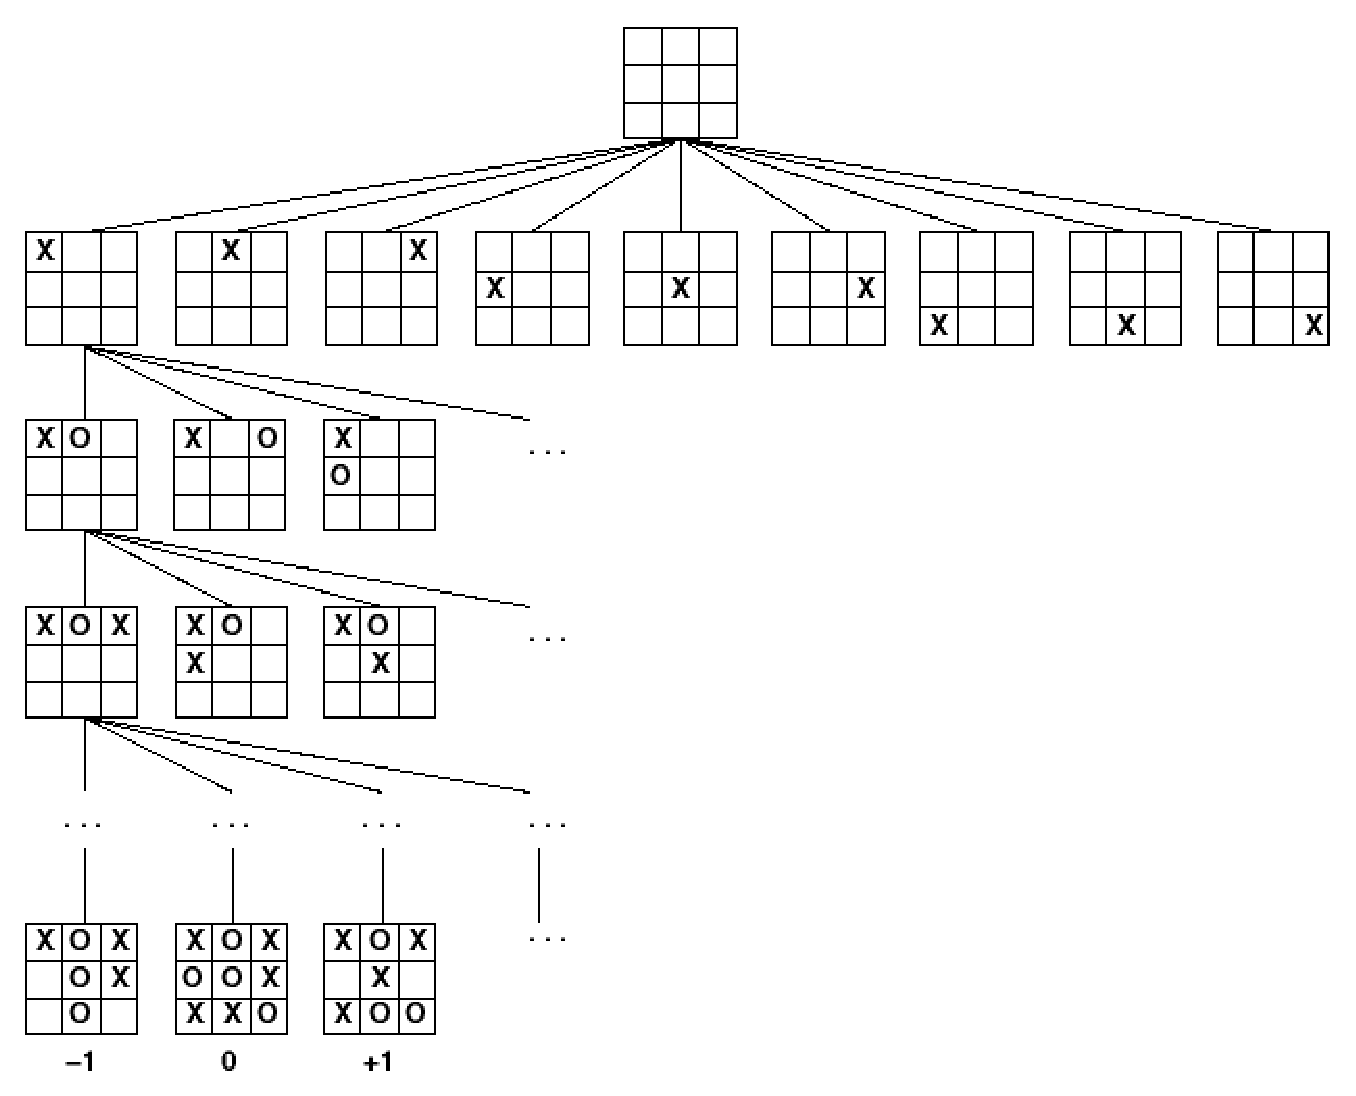
\includegraphics[scale=0.5]{contenido/cap3/imagenes/game_tree.eps}
	\caption{Árbol parcial de búsqueda para el \textit{3 en Raya}.}
	\label{fig:arbol_juego_3enraya}
\end{figure}

Los juegos a tratar son principalmente juegos bipersonales, de suma cero (si un jugador gana, el otro pierde), de información perfecta y por turnos; tal y como se definieron en el capítulo~\ref{cap:juegos} dedicado a los juegos.

\bigskip
Una vez conocido el medio en el que se desenvuelve el agente podemos completar la definición de un agente inteligente jugador de juegos.

\section{Agentes para juegos}
\label{sec:agentes_para_juegos}
En los juegos, el agente hará las veces de jugador.
Por esa razón, para referirnos a él, se utilizarán indistintamente los términos agente, agente inteligente, jugador o agente jugador.
Podemos ahora definir formalmente un agente en el contexto de los juegos.

Un \textbf{agente jugador} viene definido por los siguientes elementos:
\begin{itemize}	
	\item \textbf{El medio} \\
	El jugador se desenvuelve en el espacio de estados de un juego (representado mediante el árbol de juegos) donde otro jugador independiente (un adversario) mueve por turnos. 
	\item \textbf{Objetivos} \\
	El objetivo del agente es ganar el juego.
	\item \textbf{Percepciones} \\
	El agente es capaz de percibir el estado del juego antes de realizar cada movimiento.
	\item \textbf{Acciones} \\
	El agente es capaz de ejecutar movimientos válidos del juego.
	Pueden existir limitaciones de tiempo para realizar el siguiente movimiento.
	\item \textbf{Conocimiento} \\
	El jugador necesita una representación y una \textit{estrategia} que le permitan proponer un movimiento válido conforme a las reglas del juego.
\end{itemize}

De la sofisticación de la estrategia que use, así como de las limitaciones físicas (por ejemplo, tiempo de cálculo), dependerá la capacidad del agente para alcanzar su objetivo.

\section{Búsqueda de una estrategia ganadora}
\label{sec:busqueda_de_una_estrategia_ganadora}
Una \textbf{estrategia ganadora} es un camino (secuencia de movimientos) desde la raíz del árbol de juegos (estado inicial) hasta las hojas del árbol (estados terminales), que garantiza que el jugador gana siempre.
En la terminología introducida en la sección~\ref{sec:el_medio}, una estrategia ganadora es una solución del árbol de juegos que se corresponde con un \textbf{hipercamino solución}, es decir, un camino de arcos e hiperarcos tal que todas sus hojas son ganadoras para un jugador.

Encontrar una solución a través de una búsqueda directa desde el estado inicial hasta una posición ganadora no es factible hoy día salvo para juegos muy sencillos (como el \textit{Grundy}), ya que no es posible generar todo el árbol de búsqueda.
Incluso para un juego simple como el \textit{3 en Raya} es complejo dibujar el árbol de juegos completo.
La tabla~\ref{tab:complejidad_juegos} presentada en el capítulo~\ref{cap:juegos} muestra este hecho.
% poner tabla de juegos y complejidad en relacion al factor de ramificacion.

Por lo tanto no se puede conocer de antemano una estrategia ganadora para un jugador; y en la mayoría de los casos hay que conformarse con obtener una buena jugada a partir de una configuración dada.
Esto obliga al agente a tomar algún tipo de decisión para realizar los movimientos del juego.

\bigskip
En la siguiente sección se estudiarán las diferentes estrategias y algoritmos propuestos que usarán los agentes.

\section{Estrategias}
\label{sec:estrategias}
A continuación se estudian los algoritmos y estrategias desarrollados.
Todas las estrategias han sido incluidas en la aplicación interactiva para poder usarlas: jugar con ellas, analizarlas y compararlas.
Los algoritmos estudiados son versiones generales de los mismos con el objetivo de que sean sencillos de entender y resulten útiles para la docencia.
Versiones más sofisticadas de los algoritmos propuestos pueden ser desarrolladas e incluidas en la aplicación como se explica en el apéndice~\ref{cap:desarrollo_juegos_estrategias_heuristicos}.

%\bigskip
% PONER ESTO EN LA INTRODUCCION.
%Implementarán versiones generales de estas estrategias de forma que resulten
%sencillas de entender de cara a la docencia. Estas van desde el caso más básico
%como la estrategia aleatoria hasta algoritmos más complejos como una estrategia
%con aprendizaje u otra con redes neuronales, pasando por los clásicos
%algoritmos de evaluación minimax y poda alfa-beta, entre otros.
%Además de las estrategias que se detallan a continuación, para cada juego
%se implementará un jugador que pida el movimiento al usuario. De esta
%manera un jugador humano podrá jugar contra cualquier estrategia o incluso
%contra otro jugador humano.

\subsection{Aleatoria}
\label{ssec:aleatoria}
La estrategia más sencilla es un jugador que realice movimientos aleatorios.
Este jugador es totalmente independiente del juego.

Un agente con una estrategia aleatoria obtiene todos los posibles estados sucesores a partir del estado actual del juego y elige uno de ellos de forma aleatoria.
Esta forma de proceder es ineficiente para juegos con un factor de ramificación elevado;
pero evita que el agente deba conocer cómo se generan los estados para cada juego, ya que los estados sucesores son generados por el propio estado actual del juego, tal y como se definió en~\ref{sec:juegos_problemas_busqueda_adversario}.
Esto hace que el agente pueda jugar a cualquier tipo de juego.

Una estrategia aleatoria tampoco ayuda al agente a lograr su objetivo (ganar) de una forma directa;
pero será de gran utilidad como base para comparar el rendimiento del resto de estrategias, además de servir como estrategia oponente en los entrenamientos de los agentes que lo requieran. 

\subsection{Evaluador heurístico}
\label{ssec:evaluador_heuristico}
Un agente evaluador heurístico es capaz de evaluar heurísticamente si una situación dada le es favorable o no.

El agente emplea la siguiente estrategia de juego: \emph{dada una situación, considera todos los movimientos inmediatos, los evalúa heurísticamente y escoge el mejor.}

Esta estrategia, al contrario que la estrategia aleatoria, no es totalmente independiente del juego, pues necesita de una función de evaluación heurística que depende del tipo de juego.

Cualquier jugador que necesite de una función de evaluación heurística puede considerarse como una especialización de este agente.
El capítulo~\ref{cap:heuristicos} está dedicado a los evaluadores heurísticos que pueden usar los agentes.

%\bigskip
%La siguiente sección estudia la estrategia minimax y los agentes desarrollados que emplean dicha estrategia.

\subsection{Minimax}
\label{ssec:minimax}
Antes de presentar los agentes que emplean la estrategia minimax, se detallará el algoritmo minimax de forma general, así como la variante implementada: negamax.

\bigskip
El \textbf{algoritmo minimax} proporciona una estrategia óptima, aunque en la práctica no es factible calcularla para juegos complejos.
Una \textbf{estrategia óptima}, en un problema de búsqueda normal, es una secuencia de movimientos que conducen a un estado objetivo (un estado terminal que es ganador).
Sin embargo, en problemas de búsquedas con adversario, el otro jugador también participa y su objetivo es el mismo y opuesto al del primer jugador, por lo que deberá usar una estrategia contingente.
Podemos decir que una estrategia óptima conduce a resultados al menos tan buenos como cualquier otra estrategia cuando uno juega con un oponente infalible.

La estrategia minimax consiste en realizar un análisis desde la posición actual y generar una serie de jugadas posibles por parte de ambos jugadores.
Una vez alcanzado el nivel de profundidad deseado en el árbol de juegos se utiliza una función de evaluación que asigna valores numéricos a las posiciones finales, lo que permite, además de elegir la mejor posición, transmitir esta información hasta la posición actual que corresponde a la raíz del árbol generado. 
Minimax sólo tiene en cuenta una visión local del árbol de búsqueda.

Llamaremos al primer jugador \textit{MAX} y al segundo jugador \textit{MIN}; y etiquetaremos los niveles del árbol con \textit{MAX} y \textit{MIN} según le toque jugar a \textit{MAX} o \textit{MIN} respectivamente.

Considerando un árbol de juegos, la estrategia óptima puede determinarse examinando el valor minimax de cada nodo, que llamamos \textit{VALOR\_MINIMAX(n)}.
El valor minimax de un nodo es la utilidad (para \textit{MAX}) de estar en el estado correspondiente, asumiendo que ambos jugadores juegan óptimamente desde allí hasta el final del juego.
El valor minimax de un estado terminal es su utilidad.
Considerando una opción, \textit{MAX} prefiere mover a un estado de valor máximo, mientras que \textit{MIN} prefiere un estado de valor mínimo. 
Se define entonces el \textit{VALOR\_MINIMAX(n)} de un nodo como:
{\footnotesize
\begin{equation}
VALOR\_MINIMAX(n) = 
\left\{\begin{array}{ll}
UTILIDAD(n) & \textnormal{si \textit{n} es un estado terminal}\\
\max_{s\in Sucesores(n)} VALOR\_MINIMAX(s) & \textnormal{si \textit{n} es un estado \textit{MAX}}\\
\min_{s\in Sucesores(n)} VALOR\_MINIMAX(s) & \textnormal{si \textit{n} es un estado \textit{MIN}}\\
\end{array}\right. \label{eq:minimax}
\end{equation}
}

La figura~\ref{fig:minimax} muestra el funcionamiento del algoritmo minimax para un árbol de juegos.
Los nodos $\Box$ son <<nodos \textit{MAX}>>, en los que le toca mover a \textit{MAX}, y los nodos $\bigcirc$ son <<nodos \textit{MIN}>>.
Los nodos terminales muestran los valores de utilidad para \textit{MAX}; los otros nodos son etiquetados por sus valores minimax.

\begin{figure}[h]
	\centering
	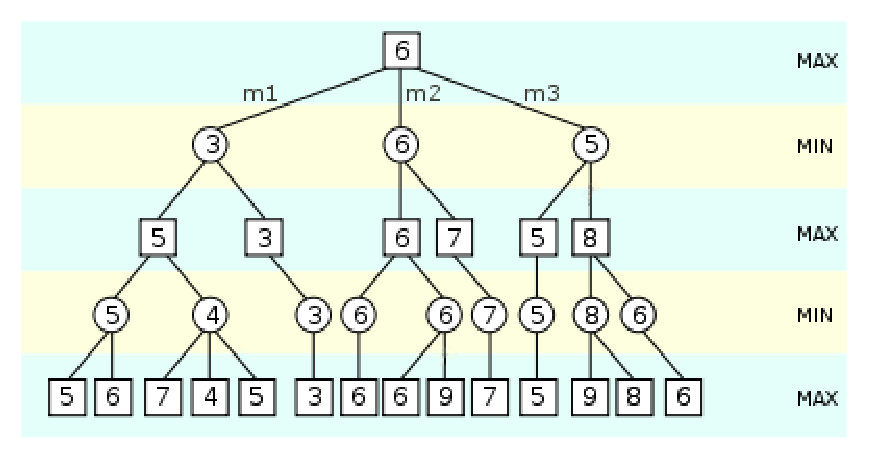
\includegraphics[scale=0.8]{contenido/cap3/imagenes/minimax.eps}
	\caption{Minimax aplicado a un árbol de juegos.}
	\label{fig:minimax}
\end{figure}

Se realiza una exploración hacia delante, generando primero el árbol completo a una determinada profundidad (cuatro en este caso), a continuación se evalúan las hojas con la función de utilidad y los valores se propagan hacia arriba de la siguiente forma:
\begin{itemize}
\renewcommand{\labelitemi}{-}
	\item Un nodo \textit{MAX} toma como valor el máximo de sus hijos.
	\item Un nodo \textit{MIN} toma como valor el mínimo de sus hijos.
\end{itemize}
Finalmente, el movimiento de \textit{MAX} es el mejor valorado de sus hijos inmediatos, que en el caso de la figura~\ref{fig:minimax} se trata del movimiento \textit{m2}.

Esta forma de proceder es más fiable que evaluar solamente los hijos inmediatos, como hacía el agente evaluador heurístico presentado en la sección~\ref{ssec:evaluador_heuristico}.
La función de utilidad que usa minimax para asignar los valores a los nodos evaluados es una función de evaluación heurística, puesto que en la mayoría de los casos los estados a evaluar no serán terminales.
Esta función se define en el capítulo~\ref{cap:heuristicos} dedicado a los evaluadores heurísticos.

El algoritmo minimax realiza una exploración primero en profundidad.
Para una búsqueda en un árbol a profundidad \textit{p} y un factor de ramificación \textit{b}, minimax evaluará $b^p$ nodos hojas.
La complejidad en tiempo del algoritmo minimax es $O(b^p)$; y la complejidad en espacio es $O(bp)$ si se generan todos los sucesores a la vez, o $O(p)$ si se generan uno por uno.
Para juegos reales, los costes de tiempo son impracticables, pero este algoritmo sirve como base para el análisis matemático de juegos y para otros algoritmos más prácticos.

Existen numerosas mejoras del algoritmo minimax original; algunas de ellas consisten en realizar:
\begin{itemize}
	\item una búsqueda en profundidad con retroceso (\textit{backtrack}),
	\item una búsqueda con profundización progresiva (\textit{algoritmos anytime}),
	\item explorar sólo la parte imprescindible del árbol (\textit{poda alfa-beta}), o
	\item almacenar información sobre los estados visitados anteriormente  y usarla cuando nos encontremos esos estados por otro camino del árbol (\textit{tablas de transposiciones}).
\end{itemize}
A continuación se detallan cada una de estas mejoras que se han implementado e incorporado a la aplicación; presentando primero la variante implementada del algoritmo minimax: negamax.

\subsubsection{Negamax}
\label{sssec:negamax}
En lugar del algoritmo minimax propiamente dicho se ha implementado una variante equivalente conocida como \textbf{negamax}.
En esta variante, cada nodo del árbol de juegos toma siempre el valor máximo de sus hijos, independientemente de que sea un nodo \textit{MAX} o \textit{MIN}.
Adicionalmente, los valores de los nodos \textit{MAX} se cambian de signo.
De este modo, es equivalente para un nodo \textit{MIN} tomar el máximo de las evaluaciones cambiadas de signo, que tomar el mínimo de las evaluaciones sin alterar.
El origen de negamax se basa en la igualdad matemática:
\begin{displaymath}
\max{(x, y)} = - \min{(-x, -y)}
\end{displaymath}

Negamax no supone una mejora directa de minimax, sino que se trata más bien del algoritmo minimax comprimido que evita tener que definir dos funciones distintas para \textit{MAX} y \textit{MIN}.
Además, se sigue teniendo el mismo problema de la complejidad que supone explorar el árbol de juegos al completo.
Para evitar esto se ha modificado la versión original de negamax dando lugar a dos agentes que emplean dos estrategias diferentes: una con profundidad máxima de búsqueda y otra con un límite de tiempo.

\subsubsection{Minimax con profundidad máxima de búsqueda}
\label{sssec:profundidad_maxima_busqueda}
El primer agente emplea una estrategia con la variante negamax y un parámetro adicional que indica la profundidad máxima de búsqueda en el árbol de juegos a partir de la posición actual.

La estrategia comienza en la posición actual y realiza una búsqueda en profundidad con retroceso (\textit{backtrack}) hasta la profundidad de búsqueda indicada.
Los sucesores son generados aleatoriamente de uno en uno y en cada paso el algoritmo se queda con el mejor movimiento en función del valor minimax devuelto.

% PONER ESTO EN DISEÑO.
%El algoritmo minimax y su variante negamax es recursivo por naturaleza y así ha sido implementado; aunque esto pueda parecer un inconveniente en cuanto a la eficiencia, el algoritmo resultante es muy fácil de entender y esto era uno de los objetivos de este proyecto, por encima de la eficiencia obtenida en los algoritmos.
%Además, una versión iterativa de los mismos no siempre supone una mejora en la eficiencia, debido al gran aumento en complejidad que supone desarrollar y gestionar una estructura temporal (por ejemplo una pila) para almacenar la información de la recursividad.

Este agente puede evaluar posiciones a una profundidad dada.
Sin embargo, incrementos lineales de profundidad pueden originar búsquedas que requieran un tiempo exponencialmente mayor.
Del mismo modo, aún sin variar la profundidad, el tiempo necesario para la búsqueda puede ser muy variable.
Normalmente el número de posibilidades al comienzo de un juego es mucho mayor que a medida que se desarrolla la partida, por lo que examinar los movimientos iniciales puede llevar un tiempo mayor.

La limitación del tiempo de cómputo puede superarse empleando un algoritmo que en cualquier momento pueda dar una solución, pero que proporcione soluciones mejores cuanto mayor sea el tiempo disponible.
Los algoritmos que presentan esta propiedad se conocen como algoritmos \textit{anytime}.
El siguiente agente, que también emplea una estrategia minimax, dispone de un límite de tiempo para realizar la búsqueda, en lugar de un límite en la profundidad máxima de búsqueda.

\subsubsection{Minimax con límite de tiempo}
\label{sssec:limite_tiempo}
El segundo agente también emplea negamax pero dispone de un tiempo limitado para realizar la búsqueda del mejor movimiento en el árbol de juegos.

Se trata de un algoritmo \textit{anytime}.
Un \textbf{algoritmo \textit{anytime}} devuelve una solución cuya calidad depende del tiempo de cómputo disponible.
El algoritmo encontrará mejores soluciones a medida que aumenta el tiempo disponible para realizar la búsqueda.

La estrategia realiza una búsqueda con retroceso y profundización progresiva (\textit{Backtrack with Iterative Deepening}.
La búsqueda dispone de una cota (profundidad máxima de búsqueda) que se incrementa automáticamente en cada iteración.
El algoritmo guarda siempre la mejor jugada inmediata para la última exploración realizada con objeto de devolverla cuando el tiempo se acabe.
En cada iteración el algoritmo comprueba el tiempo restante, terminando la búsqueda cuando este se agota.

Puede darse el caso de que el límite de tiempo sea tan pequeño que la estrategia no tenga tiempo de devolver un movimiento, en ese caso el agente acabará realizando un movimiento aleatorio.
Además, para asegurarse de devolver el mejor movimiento, la estrategia debe evaluar todos los nodos del nivel del árbol que corresponde a la cota de la iteración actual.
Si en la iteración actual no ha tenido tiempo de evaluarlos todos, devolverá el mejor movimiento obtenido en la iteración anterior.

Por simplicidad, la unidad de tiempo escogida ha sido el segundo, pues para la mayoría de juegos no tiene sentido dejar menos tiempo de cómputo al agente debido a la complejidad de los propios juegos.
Esto implica que el tiempo mínimo permitido sea de un segundo.


\bigskip
Una vez vista la estrategia básica minimax y su variante negamax, dedicaremos la siguiente sección a estudiar otra mejora de minimax: la poda alfa-beta.

\subsection{Poda alfa-beta}
\label{ssec:poda_alfa_beta}
Esta sección estudia la técnica de la poda alfa-beta como una mejora del algoritmo minimax.
También define los agentes que emplearán esta estrategia, que al igual que ocurría con minimax serán dos: uno con límite de profundidad en la búsqueda y otro con un límite en el tiempo de cómputo.

\bigskip
La \textbf{poda alfa-beta} calcula el mismo movimiento que devolvería minimax sin necesidad de examinar todos los nodos en el árbol de juegos, es decir, poda las ramas del árbol que no influyen en la decisión final.

Esta estrategia dispone de dos parámetros ($\alpha$ y $\beta$) que describen los límites sobre los valores que se propagan hacia arriba en el árbol:
\begin{itemize}
	\item $\alpha$ es el valor de la mejor opción (es decir, el valor más alto) que se ha encontrado hasta ahora en cualquiera de los estados elegidos para \textit{MAX}. 
	\item $\beta$ es el valor de la mejor opción (es decir, el valor más bajo) que se ha encontrado hasta ahora en cualquiera de los estados elegidos para \textit{MIN}.
\end{itemize}
La poda alfa-beta realiza una búsqueda primero en profundidad, con retroceso y de izquierda a derecha.
Para cada nodo se considera un intervalo de posibles valores [$\alpha$, $\beta$].
La búsqueda actualiza estos valores según recorre el árbol: actualiza el valor $\alpha$ (en los nodos \textit{MAX}) y el valor $\beta$ (en los nodos \textit{MIN}).
Cuando encuentra un nodo con un valor peor que su antecesor, la búsqueda se detiene y esa rama del árbol no se examina.
Así, se puede podar:
\begin{itemize}
\renewcommand{\labelitemi}{-}
	\item Debajo de un nodo \textit{MIN} cuando un nodo \textit{MAX} antecesor suyo tenga un valor $\alpha \geq \beta$; lo que se conoce como \textbf{corte $\alpha$}.
	\item Debajo de un nodo \textit{MAX} cuando un nodo \textit{MIN} antecesor suyo tenga un valor $\beta \leq \alpha$; lo que se conoce como \textbf{corte $\beta$}.
\end{itemize}

La figura~\ref{fig:alfabeta} muestra el funcionamiento de la poda alfa-beta para el mismo árbol de juegos de la figura~\ref{fig:minimax}.
Los nodos \textit{MAX} muestran el valor final de $\alpha$ mientras que los nodos \textit{MIN} muestran el valor final de $\beta$.
El valor minimax devuelto por la poda alfa-beta para el nodo raíz es el mismo que el valor devuelto por el algoritmo minimax y en este caso, el movimiento es también el mismo (\textit{m2}).

\begin{figure}[h]
	\centering
	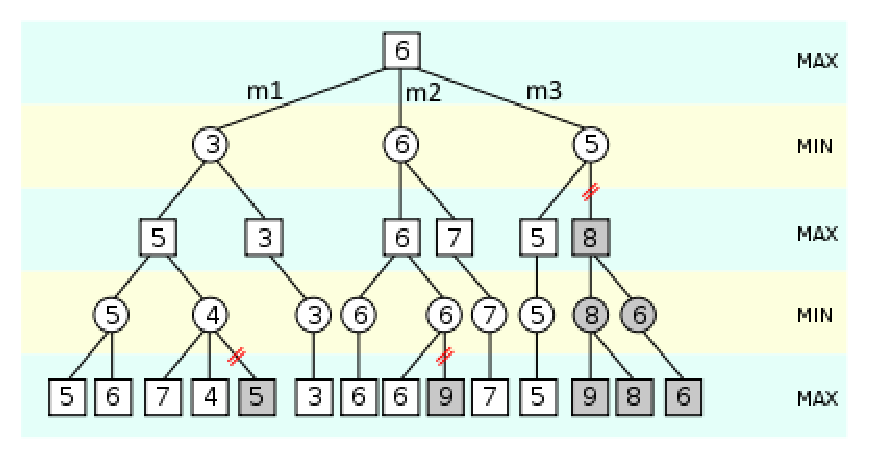
\includegraphics[scale=0.8]{contenido/cap3/imagenes/podaalfabeta.eps}
	\caption{Poda alfa-beta aplicada a un árbol de juegos.}
	\label{fig:alfabeta}
\end{figure}

En los agentes desarrollados esto no siempre es así y puede ocurrir que el mejor movimiento devuelto por minimax sea distinto del mejor movimiento devuelto por alfa-beta (pero ambos tendrán el mismo valor de evaluación); esto se debe a que los sucesores son generados en orden aleatorio y además, en el caso de que más de un estado tenga la misma evaluación, minimax cogerá el último sucesor que evalúe mientras que alfa-beta puede podar esa rama si encontró otro nodo con la misma evaluación.

La eficacia de la poda alfa-beta depende mucho del orden en el que se examinan los sucesores.
Una posible mejora del algoritmo sería examinar primero los sucesores que probablemente sean mejores.
Para una búsqueda en un árbol a profundidad \textit{p} y un factor de ramificación \textit{b}, en el mejor caso (los nodos están ordenados de mejor a peor), alfa-beta tiene que examinar $O(b^{p/2})$ nodos para escoger el mejor movimiento, en vez de $O(b^p)$ para minimax.% lo que reduce a la mitad el tiempo necesario.
En los algoritmos desarrollados donde los sucesores se examinan en orden aleatorio, el número total de nodos examinados es de $O(b^{3p/4})$.
Por último, en el peor de los casos, donde no se realiza ninguna poda, la complejidad es la misma que en minimax: $O(b^p)$.

\bigskip
A continuación se presentan los agentes que emplean la técnica de la poda alfa-beta, al igual que ocurría con minimax se trata de dos agentes con características diferentes: uno con un límite en la profundidad de búsqueda y otro con un tiempo limitado de búsqueda.

\subsubsection{Alfa-beta con profundidad máxima de búsqueda}
\label{sssec:profundidad_maxima_busqueda_alfabeta}
Este agente emplea el algoritmo negamax con poda alfa-beta incluida para realizar una búsqueda en el árbol de juegos a una profundidad máxima indicada a partir de la posición actual.

La lógica del agente es la misma que la explicada para el agente minimax con profundidad máxima de búsqueda (apartado~\ref{sssec:profundidad_maxima_busqueda}), con el incentivo de que incorpora la poda alfa-beta.

\subsubsection{Alfa-beta con límite de tiempo}
\label{sssec:limite_tiempo_alfabeta}
El segundo agente también emplea el algoritmo negamax con poda alfa-beta y dispone de un tiempo limitado para realizar la búsqueda del mejor movimiento en el árbol de juegos.

El agente tiene las mismas características que el agente minimax con límite de tiempo (descrito en el apartado~\ref{sssec:limite_tiempo}), pero incluyendo además las ventajas de la poda alfa-beta.


\bigskip
Otra mejora con respecto al algoritmo minimax original y de alfa-beta es la posibilidad de incorporar una tabla de transposición a la búsqueda.
En la siguiente sección se estudian las tablas de transposición.

\subsection{Tablas de transposición}
\label{ssec:tablas_transposicion}
Esta sección desarrolla los conceptos de \textit{transposición} y \textit{tabla de transposición} para las búsquedas en árboles de juegos.
Se presentan también los agentes que emplean esta técnica.

\bigskip
Una \textbf{transposición} es una permutación diferente de una secuencia de movimientos que termina en la misma posición.
En el árbol de juegos se trata de un estado que puede ser alcanzado por más de un camino distinto.

Los estados repetidos en el árbol de búsqueda pueden causar un aumento exponencial del coste de la búsqueda.
Es por ello que merece la pena almacenar la evaluación de ese estado en una tabla la primera vez que se encuentre, de modo que no tenga que volver a calcularse la próxima vez que se visite.
A esta tabla se le conoce como tabla de transposición.

Una \textbf{tabla de transposición} o \textbf{tabla de transposiciones} es una base de datos donde se almacenan los resultados de búsquedas previamente realizadas.
Normalmente se implementa mediante una tabla \textit{hash} de gran capacidad y se almacenan los estados previamente evaluados, hasta qué nivel se les realizó la búsqueda y qué acción se determinó para estos; aunque pueden almacenar más información si es necesario.

Se trata de una forma de reducir el espacio de búsqueda.
Cuando aparece una transposición, se busca en la tabla qué se determinó la última vez; evitando repetir de nuevo toda la búsqueda y pudiendo invertir ese ahorro de tiempo en aumentar la profundidad de búsqueda.

La utilización de una tabla de transposición puede tener un efecto espectacular en situaciones donde hay muchas posibles transposiciones como en la etapa final de los juegos (por ejemplo en el Ajedrez).
Por otra parte, el único problema de las tablas de transposiciones es su consumo en memoria.
Para que sean realmente útiles deben contener muchas posiciones y si se evalúan un millón de nodos por segundo no es práctico almacenar todos ellos en la tabla de transposición.

\bigskip
Los agentes que emplean las tablas de transposición son los mismos que se han presentado anteriormente para minimax y alfa-beta pero incorporando esta nueva característica, lo que da lugar a cuatro nuevos agentes que se presentan brevemente en los siguientes apartados.

\subsubsection{Minimax con profundidad máxima de búsqueda y tabla de transposición}
\label{sssec:minimax_profmax_tablatransposicion}
Se trata de un agente que realiza una búsqueda en el árbol de juegos mediante el algoritmo minimax, dispone de un límite en la profundidad máxima de búsqueda a partir del estado actual y cuenta con una tabla de transposición para almacenar los estados evaluados y usar la información guardada en caso de encontrar una transposición.

Para más información sobre este agente se puede consultar el agente minimax con profundidad máxima de búsqueda en la sección~\ref{sssec:profundidad_maxima_busqueda}.

\subsubsection{Minimax con límite de tiempo y tabla de transposición}
\label{sssec:minimax_limiteTiempo_tablatransposicion}
Este agente realiza una búsqueda en el árbol de juegos empleando el algoritmo minimax, dispone de un límite de tiempo para devolver el mejor movimiento y cuenta con una tabla de transposición.

La sección~\ref{sssec:limite_tiempo} contiene información sobre el agente minimax con límite de tiempo.

\subsubsection{Alfa-beta con profundidad máxima de búsqueda y tabla de transposición}
\label{sssec:alfabeta_profmax_tablatransposicion}
Este agente emplea el algoritmo minimax con poda alfa-beta incluida para realizar la búsqueda en el árbol de juegos; tiene una profundidad máxima de búsqueda y se ayuda de una tabla de transposición para evitar evaluar los estados repetidos.

En la sección~\ref{sssec:profundidad_maxima_busqueda_alfabeta} se detalla el agente alfa-beta con profundidad máxima de búsqueda, que cuenta con las mismas características que este, salvo obviamente, la tabla de transposición.

\subsubsection{Alfa-Beta con límite de tiempo y tabla de transposición}
\label{sssec:alfabeta_limiteTiempo_tablatransposicion}
El último agente también usa el algoritmo minimax con poda alfa-beta; tiene un límite de tiempo para realizar la búsqueda en el árbol y también cuenta con una tabla de transposición.

El agente alfa-beta con límite de tiempo puede consultarse en la sección~\ref{sssec:limite_tiempo_alfabeta}.

\bigskip
A continuación se describen los agentes que no necesitan de un evaluador heurístico para determinar el mejor movimiento, estos son los agentes que usan el método de Monte-Carlo y Monte-Carlo Tree Search.
Ambas estrategias son totalmente independientes del tipo de juego, ya que no necesitan de una función de evaluación heurística.

\subsection{Monte-Carlo}
\label{ssec:montecarlo}
Esta sección explica el método de Monte-Carlo aplicado a los problemas de búsqueda en árboles de juegos.
Se estudia una versión básica del mismo y se presentan los agentes que lo usan.

El \textbf{método de Monte-Carlo} consiste en realizar un número de simulaciones a partir del estado actual para decidir el próximo movimiento.

Una \textbf{simulación} es una partida al azar completa del juego desde la posición actual; es decir, partiendo del estado actual en el árbol de juegos, se realizan movimientos aleatorios hasta llegar a un estado terminal, donde se asigna el valor de utilidad (+1, -1 ó 0 si es el estado es ganador, perdedor o empate para el jugador).
Este valor es usado como la recompensa esperada que se puede obtener a partir del estado sucesor elegido.
Para estimar el valor final de un estado se toman estadísticas haciendo un promedio de las recompensas obtenidas en las simulaciones.

El método genera una lista de posibles movimientos (sucesores del estado actual) y para cada movimiento realiza miles de simulaciones (partidas al azar), obteniendo el valor de recompensa.
El movimiento con un valor de recompensa mayor es el elegido como mejor movimiento, es decir, aquel que conduce a la mejor serie de partidas al azar para el jugador actual.

La ventaja de esta técnica es que requiere poco conocimiento del entorno, pero se incrementan los requisitos computacionales (procesador y memoria).
Para que el método sea efectivo se deben realizar muchísimas simulaciones, ya que los movimientos de las simulaciones se generan al azar y es posible que una buena jugada sea evaluada erróneamente como una mala jugada.

A priori es difícil establecer de antemano un número determinado de simulaciones, por lo que se suele dejar un tiempo máximo para realizar las simulaciones.

\bigskip
Los siguientes apartados presentan dos agentes que usan el método de Monte-Carlo: uno con un número determinado de simulaciones y otro con un límite de tiempo para realizar las simulaciones.

\subsubsection{Monte-Carlo con número de simulaciones fijas}
\label{sssec:montecarlo_simulaciones}
El jugador Monte-Carlo más simple es aquel que tiene un número de simulaciones determinado.

Partiendo del estado actual juega el número de partidas indicadas para evaluar el mejor movimiento.
Para cada sucesor del estado actual se realiza un número diferente de simulaciones, pues estos también son elegidos aleatoriamente.
El número de simulaciones debe ser suficientemente grande para asegurarse de que se realizan aproximadamente el mismo número de simulaciones para cada posible movimiento.
Si \textit{N} es el número total de simulaciones a realizar y \textit{p} es el número de sucesores del estado actual, se espera que se realicen $p/N$ simulaciones para cada movimiento.
Esto sólo se cumple cuando \textit{N} tiende a infinito.

Asignar de antemano un número determinado de simulaciones es una tarea complicada.
Juegos con un espacio de estados mayor requieren mayor número de simulaciones, pero el tiempo de cómputo necesario también es mucho mayor.

\bigskip
El siguiente agente incorpora un límite de tiempo para realizar las simulaciones.

\subsubsection{Monte-Carlo con límite de tiempo}
\label{sssec:montecarlo_limiteTiempo}
El segundo agente que emplea el método de Monte-Carlo dispone de un límite de tiempo para realizar simulaciones.

Se trata de otro algoritmo \textit{anytime}; devuelve mejores soluciones a medida que aumenta el tiempo disponible para realizar la búsqueda, en este caso para realizar las simulaciones.

Asignar un tiempo límite para Monte-Carlo tampoco es tarea sencilla pues no conocemos el tiempo necesario que necesita cada simulación.
La simulaciones deben completarse totalmente para que sean válidas.
No tiene sentido dejar un sólo segundo para realizar simulaciones si cada simulación dura más de un segundo.
En ese caso el tiempo disponible del agente se extenderá hasta el tiempo necesario para terminar la simulación.

Por simplicidad, al igual que ocurre con la estrategia minimax con tiempo limitado (seccion~\ref{sssec:limite_tiempo}), la unidad de tiempo escogida ha sido el segundo.

\bigskip
Una vez presentado el método básico de Monte-Carlo, se explica una versión mejorada del mismo: Monte-Carlo Tree Searh.
También se describen los agentes que usan esta nueva versión.

\subsection{Monte-Carlo Tree Search}
\label{ssec:monteCarloTreeSearch}
Esta sección detalla la estrategia Monte-Carlo Tree Search, basada en el método tradicional de Monte-Carlo explicado en la sección anterior.
Se describen también los dos agentes desarrollados que usan esta técnica.

\bigskip
\textbf{Monte-Carlo Tree Search} (MCTS a partir de ahora) consiste en realizar un número de simulaciones a partir del estado actual para decidir el próximo movimiento, igual que hace el método básico de Monte-Carlo; pero dispone además de un árbol propio para almacenar la información obtenida en las simulaciones y poder usarla para mejorar las propias simulaciones y por tanto la decisión final.

Para no confundir el árbol de búsqueda de los propios juegos con el árbol de búsqueda que emplea el método MCTS llamaremos a este último: árbol de Monte-Carlo (árbol MC).

Antes de cada simulación, MCTS realiza primero una búsqueda en el árbol de juegos a partir de la posición actual hasta encontrar un nodo que no se encuentre en el árbol MC (inicialmente el árbol MC está vacío).
Para realizar esta búsqueda se utiliza una estrategia o política basada en la información almacenada en el árbol MC.
El nuevo estado encontrado se añade al árbol MC y a partir de esa posición se realiza una simulación completa hasta el final de la partida, obteniendo el valor de utilidad del estado terminal.
Con el valor de utilidad obtenido se actualiza la información de los estados visitados en el árbol MC durante la simulación.
\begin{figure}[h]
	\centering
	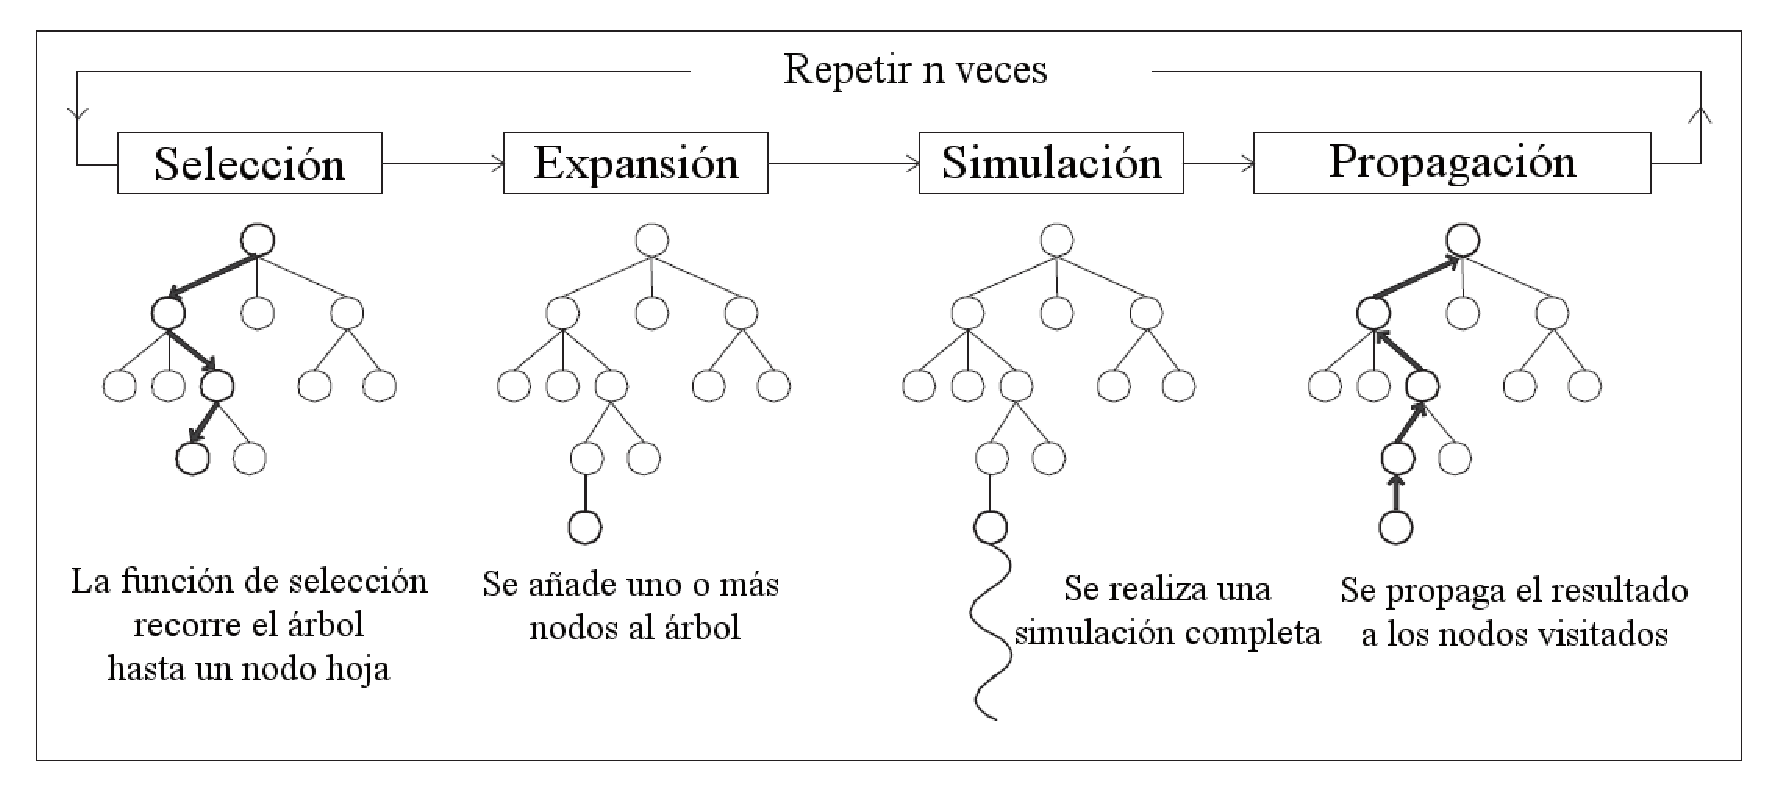
\includegraphics[scale=0.45]{contenido/cap3/imagenes/mcts1.eps}
	\caption[Fases del algoritmo Monte-Carlo Tree Search.]%
	{Fases del algoritmo Monte-Carlo Tree Search. (Imagen adaptada de \citeref{MCTS}.)}
	\label{fig:mcts1}
\end{figure}
La figura~\ref{fig:mcts1} muestra este proceso, que se puede dividir en cuatro fases:
selección, expansión, simulación y propagación.
Antes de detallar cada una de estas fases conviene definir la información que almacenará el árbol MC en cada nodo.

Sea \textit{s} el estado actual, el nodo correspondiente en el árbol MC contiene tres valores:
\begin{itemize}
	\item Número total de simulaciones realizadas desde el estado \textit{s}, que denotamos como \textit{N(s)}.
	\item Número total de simulaciones en las que se selecciona el movimiento \textit{a} desde el estado \textit{s}, que llamamos \textit{N(s,a)}.
	\item El valor Monte-Carlo del estado (valor MC), representado por \textit{Q(s,a)}, es el resultado promedio de todas las simulaciones realizadas en las que se seleccionó el movimiento \textit{a} en el estado \textit{s}:
	\begin{displaymath}
	Q(s,a)=\frac{1}{N(s,a)}\sum_{i=1}^{N(s)}\mathds{I}_i(s,a)z_i
	\end{displaymath}
	donde $z_i$ es el valor de utilidad devuelto por la \textit{i}-ésima simulación, y $\mathds{I}_i(s,a)$ es un indicador que vale 1 si el movimiento \textit{a} fue seleccionado en el estado \textit{s} durante la simulación \textit{i} y 0 en otro caso.
	Nótese que $N(s,a) = \sum_{i=1}^{N(s)}\mathds{I}_i(s,a)$.
\end{itemize}

La información almacenada puede variar dependiendo de la estrategia de selección que se use en la primera fase, aunque aquí se ha usado la información genérica que se puede obtener mediante las simulaciones, es decir, sin emplear conocimiento experto sobre el entorno.

A continuación se detalla cada una de las fases del algoritmo MCTS:
\begin{enumerate}
	\item \textbf{Selección} \\
	Partiendo del estado actual, se realiza una búsqueda en el árbol de juegos hasta encontrar un nodo que no está en el árbol MC.
	Los movimientos realizados en esta búsqueda están elegidos acorde a la información almacenada en el propio árbol MC, siguiendo una determinada estrategia.
	
La estrategia elegida debe mantener un equilibrio entre explotación y exploración.
Se puede seleccionar en cada paso el mejor movimiento, lo que favorecerá la explotación; pero por otro lado, los movimientos menos prometedores todavía tienen que ser explorados a mayor profundidad, debido a la incertidumbre de la evaluación, lo que favorecería la exploración.

En función de la estrategia escogida, obtendremos diferentes versiones del algoritmo MCTS.
Al final de la sección se citan algunas extensiones de MCTS.

Usaremos una estrategia conocida como \textit{optimism in the face of uncertainty}\footnote{Puede traducirse como \textit{optimismo frente a la incertidumbre}.}, que favorece los movimientos con un valor más alto pero permite a su vez explorar aquellas acciones que todavía no han sido suficientemente exploradas.
Para ello, definimos $Q^\oplus(s,a)$ como el valor del movimiento \textit{a} desde el estado actual \textit{s} (valor MC) con una bonificación adicional que será más alta para los movimientos menos visitados:
\begin{displaymath}
Q^\oplus(s,a) = Q(s,a) + c\sqrt{\dfrac{\log N(s)}{N(s,a)}}
\end{displaymath}
donde \textit{c} es una constante de exploración con valores reales en el intervalo [0,1] y \textit{log} es el logaritmo natural (base \textit{e}).

El movimiento elegido, que llamamos $a^\ast$, será aquel que maximize el valor $Q^\oplus(s,a)$:
\begin{displaymath}
a^\ast = \max_a{Q^\oplus(s,a)}
\end{displaymath}

	\item \textbf{Expansión} \\
	Cuando se encuentra un estado que no aparece en el árbol MC, este se añade como un nuevo nodo.
	De esta forma el árbol se expande un nodo en cada simulación.

Una variante puede ser añadir al árbol MC cada estado que se visite en la búsqueda, aunque en la práctica, para reducir los requisitos de memoria, no se añaden todos los nodos en cada simulación.
Normalmente, sólo se añade un nodo al árbol MC en cada simulación: el primer nodo encontrado que no esté presente en el árbol MC.
Si aún así la limitación de la memoria supone un problema, es posible realizar varias simulaciones antes de añadir un nuevo nodo al árbol MC; o incluso podar antiguos nodos del árbol MC a medida que la búsqueda progresa.

	\item \textbf{Simulación} \\
A partir del nuevo estado almacenado en el árbol MC se realiza una simulación completa de la partida siguiendo la estrategia por defecto, esto es, realizando movimientos aleatorios hasta el final del juego.
Después se asigna el valor de utilidad \textit{z} al estado terminal: +1 si es ganador para el jugador, -1 si es perdedor y 0 si es empate.

%En un juego no todos los posibles movimientos tienen la misma probabilidad de jugarse
Obviamente, también puede emplearse en esta fase otra estrategia distinta para elegir los posibles movimientos, como una función heurística que asigne valores más altos a aquellos movimientos que tienen más probabilidad de ser jugados o que parecen más prometedores; pero esta mejora se sale de los objetivos del proyecto por lo que los agentes desarrollados usan la estrategia por defecto para esta fase.

	\item \textbf{Propagación} \\
	Una vez realizada la simulación, se actualiza la información de cada nodo en el árbol MC en función del valor de utilidad obtenido:
	\begin{displaymath}
		\begin{array}{l}
		N(s) \leftarrow N(s) + 1 \\
		N(s,a) \leftarrow N(s,a) + 1 \\ 
		Q(s,a) \leftarrow Q(s,a) + \dfrac{z - Q(s,a)}{N(s,a)} \\
		\end{array}
	\end{displaymath}

\end{enumerate}

El movimiento final seleccionado por MCTS en el estado actual será el movimiento mejor valorado en el árbol MC, es decir, el movimiento \textit{a} con un valor MC mayor.

La figura~\ref{fig:mcts2} muestra cinco simulaciones de MCTS en las que se va construyendo el árbol MC.
Se trata de una versión simplificada del algoritmo. 
Siguiendo con la misma terminología usada en minimax, los nodos de color negro corresponden a nodos \textit{MAX}, los blancos a \textit{MIN}.
Cada simulación obtiene un valor de utilidad (en el caso de la figura~\ref{fig:mcts2} el valor es 1 si gana \textit{MAX} y 0 si gana \textit{MIN}).
En cada simulación se añade un nuevo nodo al árbol y se actualiza el valor de cada nodo en el árbol con el valor de utilidad; también se actualiza el número de veces que se ha seleccionado cada nodo.
\begin{figure}[h]
	\centering
	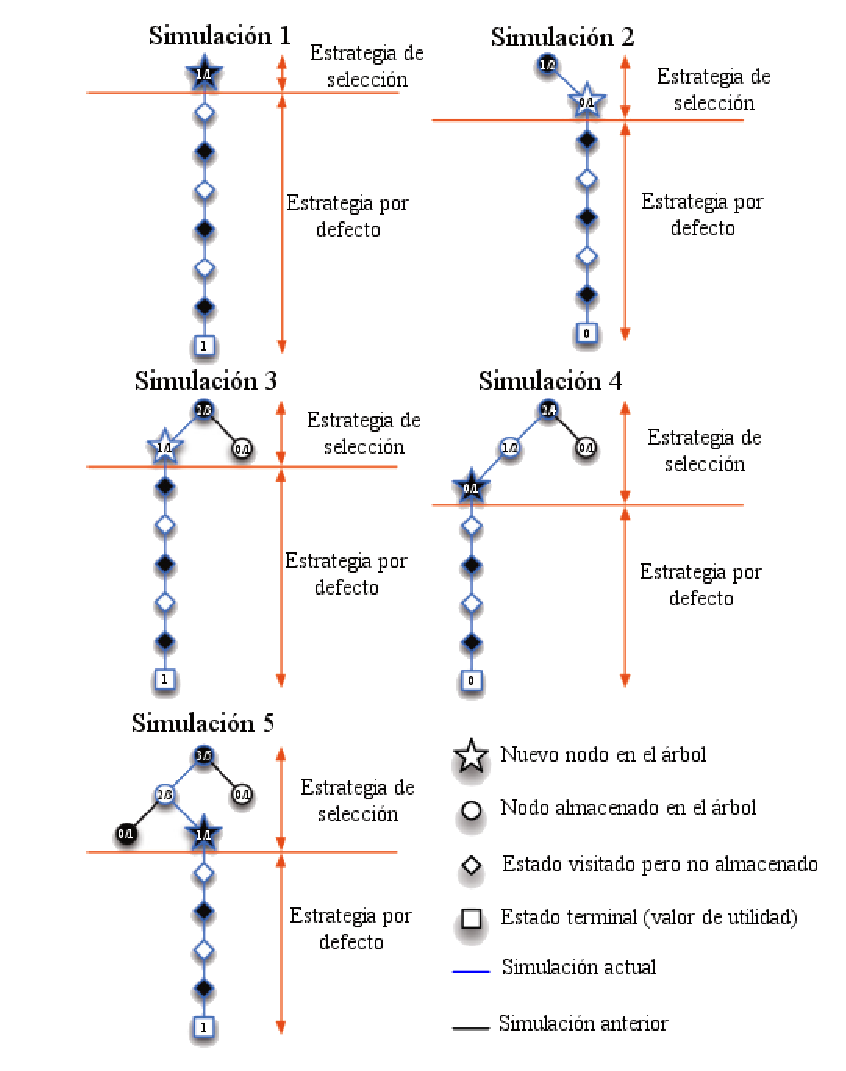
\includegraphics[scale=1]{contenido/cap3/imagenes/mcts2.eps}
	\caption[Cinco simulaciones de Monte-Carlo Tree Search.]%
	{Cinco simulaciones de Monte-Carlo Tree Search. (Imagen adaptada de \citeref{MCTS2}.)}
	\label{fig:mcts2}
\end{figure}
A medida que el árbol MC crece con cada simulación, los valores de los nodos se aproximan al valor minimax real y por tanto la estrategia basada en las simulaciones también se aproxima a la estrategia óptima de minimax.

\clearpage	% le dice a Latex que suelte todas las figuras en una página y comience una página nueva (detallado en los apuntes de los indios).

\bigskip
A continuación se presentan brevemente cuatro extensiones de MCTS en función de la estrategia elegida en las fases de selección y simulación.

\subsubsection{Extensiones de Monte-Carlo Tree Search}
\label{sssec:extensiones_MCTS}
El rendimiento de MCTS puede mejorarse significativamente si se incorpora información del dominio a la estrategia usada en la fase de selección o incluso a la estrategia por defecto usada en la fase de simulación.
Existen varias extensiones de MCTS basadas en la estrategia elegida para ambas fases, algunas extensiones son:
\begin{itemize}
	\item \textbf{\textit{Greedy MCTS}} \\
	La versión más básica de MCTS usa una estrategia \textit{best-first} (primero el mejor) que favorece la explotación frente a la exploración en la fase de selección.
A este algoritmo se le conoce como \textit{greedy MCTS}.
	\item \textbf{Algoritmo \textit{UCT}} \\
	El algoritmo \textit{UCT} (\textit{Upper Confidence bounds applied to Trees}, traducido como \textit{límites superiores de confianza aplicados a los árboles}). 
Usa el principio \textit{optimism in the face of uncertainty} que puede usarse para explorar el árbol de forma eficiente, ya que favorece a los movimientos con mayor valor potencial.
	Nuestra versión MCTS desarrollada se basa en este algoritmo.
	\item \textbf{\textit{Heuristic MCTS}} \\
	Utiliza funciones heurísticas con información del dominio para inicializar los valores de las nuevas posiciones en el árbol MC.
	\item \textbf{\textit{MC-RAVE}} \\
	Utiliza el algoritmo \textit{RAVE} (\textit{Rapid Action Value Estimation}), que mejora el método original compartiendo los valores de diferentes subárboles del árbol MC, por ejemplo en el caso de las transposiciones.
\end{itemize}
\citeref{MCTS2} contiene información detallada sobre estas extensiones de MCTS.

\bigskip
Explicada la estrategia MCTS, se presentan a continuación los agentes que la usan; al igual que ocurrió con el método básico de Monte-Carlo se trata de dos agentes: uno con un número de simulaciones fijado de antemano y otro con un límite de tiempo.

\subsubsection{Monte-Carlo Tree Search con número de simulaciones fijas}
\label{sssec:montecarloTreeSearch_simulaciones}
El primer agente que usa MCTS realiza un número de simulaciones determinado.

Partiendo del estado actual, ejecuta el ciclo de cuatro fases presentado anteriormente tantas veces como indique el número de simulaciones asignado.
Establecer el número de simulaciones en MCTS es aún más difícil que para el agente Monte-Carlo básico porque ahora cada simulación necesita más tiempo para llevarse a cabo debido a que debe gestionar el árbol MC.

Por otro lado, el agente dispone de una opción que permite reutilizar el árbol MC de un movimiento para el siguiente, ya que los valores del árbol son válidos de un movimiento a otro.
Esto permite mejorar la evaluación de los movimientos a medida que el agente juega la partida, a costa de incrementar los recursos necesarios (en memoria y tiempo) para manejar el árbol MC.
Recordemos que el árbol se expande un nodo en cada simulación.

Este agente tiene también un parámetro perteneciente a la constante de exploración \textit{c} que se vio en la fase de selección.
El parámetro permite ajustar la estrategia de selección favoreciendo la exploración (valores próximos a 1) o la explotación (valores próximos a 0).

El último agente también usa MCTS para evaluar el mejor movimiento, pero esta vez dispone de un tiempo limitado para devolver el movimiento.

\subsubsection{Monte-Carlo Tree Search con límite de tiempo}
\label{sssec:montecarloTreeSearch_limiteTiempo}
Este agente usa MCTS con un límite de tiempo para realizar las simulaciones, esto es, las iteraciones completas de cuatro fases de MCTS (selección, expansión, simulación y propagación).

Las iteraciones deben completarse totalmente para que sean válidas; de ahí que asignar el límite de tiempo no sea una tarea trivial.
Si cada iteración necesita más tiempo del disponible, el tiempo límite del agente se extenderá hasta completar la última iteración.
El límite de tiempo viene expresado en segundos al igual que el resto de jugadores con límite de tiempo que se han desarrollado.

Este agente también cuenta con la opción de reutilizar el árbol MC de un movimiento a otro; y también tiene parámetro para ajustar el nivel de exploración en la fase de selección.


